\documentclass[conference]{IEEEtran}

\usepackage{cite}
\usepackage{amsmath,amssymb,amsfonts}
\usepackage{graphicx}
\usepackage{textcomp}
\usepackage{xcolor}
\usepackage{booktabs}
\usepackage{array}
\usepackage[hidelinks]{hyperref}
\usepackage{balance}

\hypersetup{
  pdfauthor={Anonymous},
  pdftitle={Graph-Grounded Template Generation for Layered Instruction Fine-Tuning of Small Language Models in Cyber Threat Intelligence},
  pdfsubject={Double-blind conference submission},
  pdfkeywords={small language models, cyber threat intelligence, vulnerability management, layered instruction fine-tuning, knowledge graphs, data provenance}
}

\begin{document}
\bstctlcite{BSTcontrol}

\title{Graph-Grounded Template Generation for Layered Instruction Fine-Tuning of Small Language Models in Cyber Threat Intelligence}

\author{\IEEEauthorblockN{Anonymous Authors}}

\maketitle
\pagestyle{plain}
\thispagestyle{plain}

\begin{abstract}
Vulnerability response in security operations is a chain of mapping decisions: a newly disclosed CVE must be scored for severity and exploitability, traced to its weakness class and the adversary techniques it enables, and linked to mitigations and detections before a patch or compensating control is scheduled. Because the asset and exposure context behind these decisions often cannot leave the organization, locally served small language models (SLMs) are attractive, but only if their outputs land on the correct catalog identifier and their training targets are traceable to source intelligence. We present an SLM specialization workflow built on \emph{Ariadne}, a versioned Neo4j graph joining twelve public threat and vulnerability intelligence sources (e.g., NVD, CISA KEV, EPSS, CWE, ATT\&CK), and \emph{Sophia}, a template engine that materializes each instruction target by executing a typed graph query. Layered instruction fine-tuning of Qwen2.5-32B-Instruct, with a checkpoint retained after each layer, raises attack-technique extraction from 18.2 to 65.8, mitigation selection from 7.6 to 62.5, and the three-benchmark mean from 57.7 to 65.0 (95\% bootstrap interval 64.1--66.0), while CyberSOCEval is unchanged and MMLU-Pro falls 11.6 points. Checkpoint audits show that a SOC-oriented layer collapses canonical threat-actor attribution and shifts CVSS errors into Attack Vector, Privileges Required, and Scope, fields that weigh heavily in remediation priority, and that exact training--evaluation fact overlap does not explain the mapping gains.
\end{abstract}

\begin{IEEEkeywords}
small language models, cyber threat intelligence, vulnerability management, layered instruction fine-tuning, knowledge graphs, data provenance, catastrophic interference
\end{IEEEkeywords}

\section{Introduction}
For each newly disclosed CVE, vulnerability-response analysts in a security operations center (SOC) join intelligence from separate catalogs: the NVD CVSS vector; exploitation likelihood from EPSS~\cite{jacobs2021epss} and confirmed exploitation from the CISA Known Exploited Vulnerabilities (KEV) catalog; public exploit code; the CWE weakness and CAPEC attack patterns behind the flaw; the ATT\&CK techniques it enables; and the mitigations, D3FEND countermeasures, and Sigma detections that address them. Combined with private context (asset inventory, scanner findings, exposure, business criticality), these joins yield a risk assessment and a mitigation plan (patch now, compensate, or add detection until a maintenance window) that drives patch prioritization, deployment, and verification~\cite{nist80040r4}.

Each join maps free text into a controlled vocabulary, and near-misses are costly: a parent ATT\&CK technique in place of the sub-technique points detection engineering at the wrong telemetry; a related but incorrect CWE suggests the wrong compensating control; a wrong CVSS Attack Vector moves a vulnerability between remediation tiers; a misnormalized threat actor misdirects hunting; and an unparseable answer breaks downstream ticketing and orchestration. CTIBench~\cite{ctibench} and a public benchmark anonymized here as \emph{Benchmark A}~\cite{anonbench} evaluate these mappings.

That private context, along with licensed intelligence under sharing restrictions, is exactly what contractual, confidentiality, and data-residency obligations keep away from hosted APIs, favoring locally served open-weight models. We use \emph{small language model} (SLM) operationally for such locally specialized models, not as a parameter threshold: the primary base is 32B, with 8B, 14B, and sparse 30B-class transfer ports.

Specializing an SLM to these schemas raises two engineering problems. First, a recommendation that justifies an emergency change or a patch exception must be traceable, yet targets synthesized by another language model are hard to trace to a source fact. Ariadne joins twelve such public sources into a versioned graph; Sophia obtains each CTI target by executing a typed query over it and deterministically rendering the bindings. Private assets and findings fit the same schema but are not used here. Second, a single final score hides when specialization for one SOC role degrades another, so \emph{layered instruction fine-tuning} (IFT) retains a checkpoint after each of four layers: catalog mapping, attribution, SOC-style response, and recalibration.

The contribution is the construction and audit path, not a new optimizer or loss: (i) Ariadne and (ii) Sophia, whose supervised target is the deterministic rendering of an executed graph query; (iii) layered IFT with retained checkpoints for diagnosing interference; (iv) a 13-gram, entity, and gold-fact overlap audit; and (v) an evaluation with item-level bootstrap intervals, error taxonomies, and cross-architecture ports.

Training deliberately targets Benchmark A's schemas, and its development team overlaps with this study, so identifying details are masked. We evaluate the mappings that feed risk assessments and mitigation plans, not end-to-end patch planning over private telemetry. The final checkpoint does not improve CyberSOCEval, lowers MMLU-Pro, and errs more often on CVSS reachability fields than earlier checkpoints (Table~\ref{tab:vsp}); retained checkpoints show observed transitions, not causal ablations. Code is cited through an anonymized artifact~\cite{anonartifact}.

\section{Problem Formulation and Related Work}
\subsection{Inputs, Outputs, and Provenance}
Let $G_t=(V_t,E_t,A_t)$ be a versioned CTI graph at snapshot $t$, comprising typed entities, relationships, and attributes. A Sophia template $\tau$ specifies a typed query $q_\tau$, constraints, and rendering functions. For a returned binding $b\in q_\tau(G_t)$, Sophia constructs
\begin{equation}
 r_{\tau,b}=\left(i_\tau(b),x_\tau(b),y_\tau(b)\right),
\end{equation}
\begin{equation}
 y_\tau(b)=\operatorname{render}_\tau\left(q_\tau(G_t),b\right),
\end{equation}
where $i$ is the instruction, $x$ the optional question or context, and $y$ the supervised target. An audit links a generated row to its template, graph snapshot, and bound public identifiers. In the released build artifacts, a per-row template identifier and source tag supplement the three-field Alpaca representation; the training row alone is not a complete immutable provenance manifest.

The resulting model $p_\theta(y\mid i,x)$ is optimized with ordinary next-token cross-entropy. For layer $s$ with dataset $D_s$,
\begin{equation}
 \mathcal{L}_s(\theta)=-\sum_{(i,x,y)\in D_s}\sum_{j=1}^{|y|}\log p_\theta(y_j\mid i,x,y_{<j}),
\end{equation}
with the preceding checkpoint initializing the next layer. No new optimizer, loss, or inference architecture is introduced. Data, ordering, sequence length, packing, and learning rate all change across the configured treatment, so a layer transition is not an isolated causal estimate of any one variable.

\subsection{Security Instruction Tuning and Knowledge Graphs}
Instruction fine-tuning adapts pretrained models using instruction--response examples. FLAN demonstrated transfer to unseen instruction-formulated tasks~\cite{wei2022flan}; InstructGPT combined supervised demonstrations with preference-based training~\cite{ouyang2022training}; and subsequent work studied scaling instruction mixtures~\cite{chung2024scaling}. Domain-adaptive continued training further motivates separating broad domain absorption from narrow task behavior~\cite{gururangan2020dont}.

Security-specific instruction work includes CyberPal.AI, whose SecKnowledge pipeline combines expert-defined schemas, structure-driven generation, BRON graph paths, and LLM-augmented content generation~\cite{levi2025cyberpal}; subsequent work develops cybersecurity-expert SLMs using an enriched instruction pipeline with expert steering and LLM-driven multi-step grounding~\cite{levi2025slm}. SEvenLLM builds a bilingual CTI instruction corpus and companion evaluation benchmark~\cite{ji2024sevenllm}, while CyberBench presents a multi-task cybersecurity benchmark together with instruction-tuned CyberInstruct models~\cite{liu2024cyberbench}. These systems motivate domain-specific supervision, but they do not make every generated training label the deterministic result of an executed typed graph query.

CTI knowledge graphs address a related but distinct problem. Open-CyKG constructs an open cyber-threat knowledge graph from unstructured reports~\cite{sarhan2021opencykg}. That work concerns how facts enter a graph; This work primarily concerns how a populated graph is projected into IFT targets. Extraction quality and target-materialization quality should not be conflated: a Sophia target is traceable to its bound graph data, but the graph can still contain incomplete, stale, or misinterpreted source facts.

\begin{table*}[t]
\caption{Positioning against closely related security instruction-tuning systems. ``Partial'' indicates structured schemas, graph paths, or grounding traces for portions of the pipeline without making every generated label the deterministic result of an executed typed graph query.}
\label{tab:related}
\centering
\scriptsize
\setlength{\tabcolsep}{3pt}
\begin{tabular}{@{}p{0.15\textwidth}p{0.19\textwidth}p{0.19\textwidth}p{0.17\textwidth}p{0.20\textwidth}@{}}
\toprule
System & Graph-grounded targets & LLM-generated training text & Retained layer checkpoints & Provenance of a training label \\
\midrule
CyberPal.AI / SecKnowledge~\cite{levi2025cyberpal} & Partial: expert schemas and BRON graph paths for subsets & Yes: content-grounded LLM augmentation & Multi-phase data generation; retained training-stage checkpoint analysis not reported & Structured source/schema traces; some path explanations are LLM-generated \\
Cybersecurity-expert SLMs~\cite{levi2025slm} & Partial: LLM-driven multi-step grounding & Yes: enriched reasoning traces & Data-enrichment and fine-tuning pipeline; layer effects not isolated & Enriched traces with expert-in-the-loop steering \\
This work & Yes: typed Ariadne queries materialize every Sophia CTI row & No for Sophia targets; auxiliary general mixtures are external & Yes: Core, +TAA, CSE, and recalibration checkpoints retained and evaluated & Row resolves to template, graph binding, and public-source keys \\
\bottomrule
\end{tabular}
\end{table*}

\subsection{Technical Requirements and Non-Goals}
The system seeks four separable properties: source-resolvable supervision, controllable coverage of CTI schemas, inspectable specialization trade-offs, and local serving of the resulting checkpoint. A target consistent with Ariadne can still be wrong if a source record is incomplete, a graph relationship is misinterpreted, or the snapshot is stale. Similarly, graph-grounded training does not guarantee graph-faithful answers at inference time; runtime retrieval, constrained decoding, output verification, and human approval are separate mechanisms.

The evaluation concerns structured public-CTI tasks. It does not establish reliable handling of arbitrary private telemetry, autonomous containment, legal or regulatory interpretation, secure-code generation, or production incident attribution. A benchmark score is not an operational acceptance test. Deployment should be limited to validated task types with schema checks, source verification, abstention or escalation outside scope, and human review where decisions are consequential.

\section{Ariadne and Sophia: Graph-Grounded IFT Data}
\subsection{Ariadne: Source and Refresh Boundaries}
Ariadne is the populated Neo4j substrate. The reported configuration integrates twelve public CTI sources: ATT\&CK~\cite{strom2018attack}, ENGAGE, CAPEC, CWE, D3FEND, CVE, NVD, CISA KEV, FIRST EPSS, Sigma, ExploitDB, and PoC-in-GitHub. The resulting graph contains approximately 280,000 nodes and 480,000 relationships. These are snapshot sizes, not a statement that all public CTI is covered. Bounded catalogs are loaded in full, while several high-churn vulnerability and exploitation feeds are scoped to 2024 onward. EPSS and the current-year NVD feed are refreshed routinely, whereas other inputs can remain cached until an explicit refresh. Dataset freshness must therefore be assessed from per-source versions and acquisition times.

Construction follows dependency order: controlled vocabularies are loaded before vulnerability overlays and exploit references, and identifiers support idempotent population. Source keys alone are insufficient for exact replay if the corresponding source record or graph snapshot has changed. The proper unit of provenance is therefore not merely an identifier, but the identifier plus the source/version context in which the row was materialized.

\subsection{Sophia: Typed-Query Template Materialization}
Sophia parses a declarative template, executes its typed graph query, binds returned entities and relationships, and renders an instruction record. Templates support property access, relationship traversal, list expansion, hidden bindings, source disambiguation, and equality or inequality constraints. An abbreviated pattern for vulnerability-chain correlation is:
\begin{quote}\small
Question: Correlate CVE, CWE, and CAPEC for one vulnerability chain.\\
Answer: CVE \{cve:CVE.id\} impacts CAPEC \{cap:cve.impacts$>$CAPEC.name\} and is categorized as weakness \{cwe:cve.problemType$>$Weakness.name\}.\\
Constraint: \texttt{force cwe.id=cwe2.id}.
\end{quote}
The hidden equality constraint forces two traversals to resolve to the same weakness identifier. A reviewer can therefore inspect the graph binding rather than trust a separately synthesized explanation. Negative constraints can produce examples distinguishing graph-supported from unsupported associations, but absence of an edge in an incomplete CTI graph is not necessarily evidence that the relationship is false in the world. Such negatives must be interpreted relative to the declared graph and closed-world assumption.

The generation workflow parses template manifests, materializes bindings, balances and deduplicates rows, applies contamination checks and license gates, and serializes Alpaca-format JSON. Schema tests detect references to absent labels, relationships, or properties; they do not replace semantic review of source mappings. This distinction is important to the paper's provenance claim: Sophia provides a deterministic query-to-target path, not a universal guarantee that every upstream fact is correct.

\begin{figure*}[t]
    \centering
    % Redrawn, double-blind version of the manuscript pipeline figure; file is included in figures/.
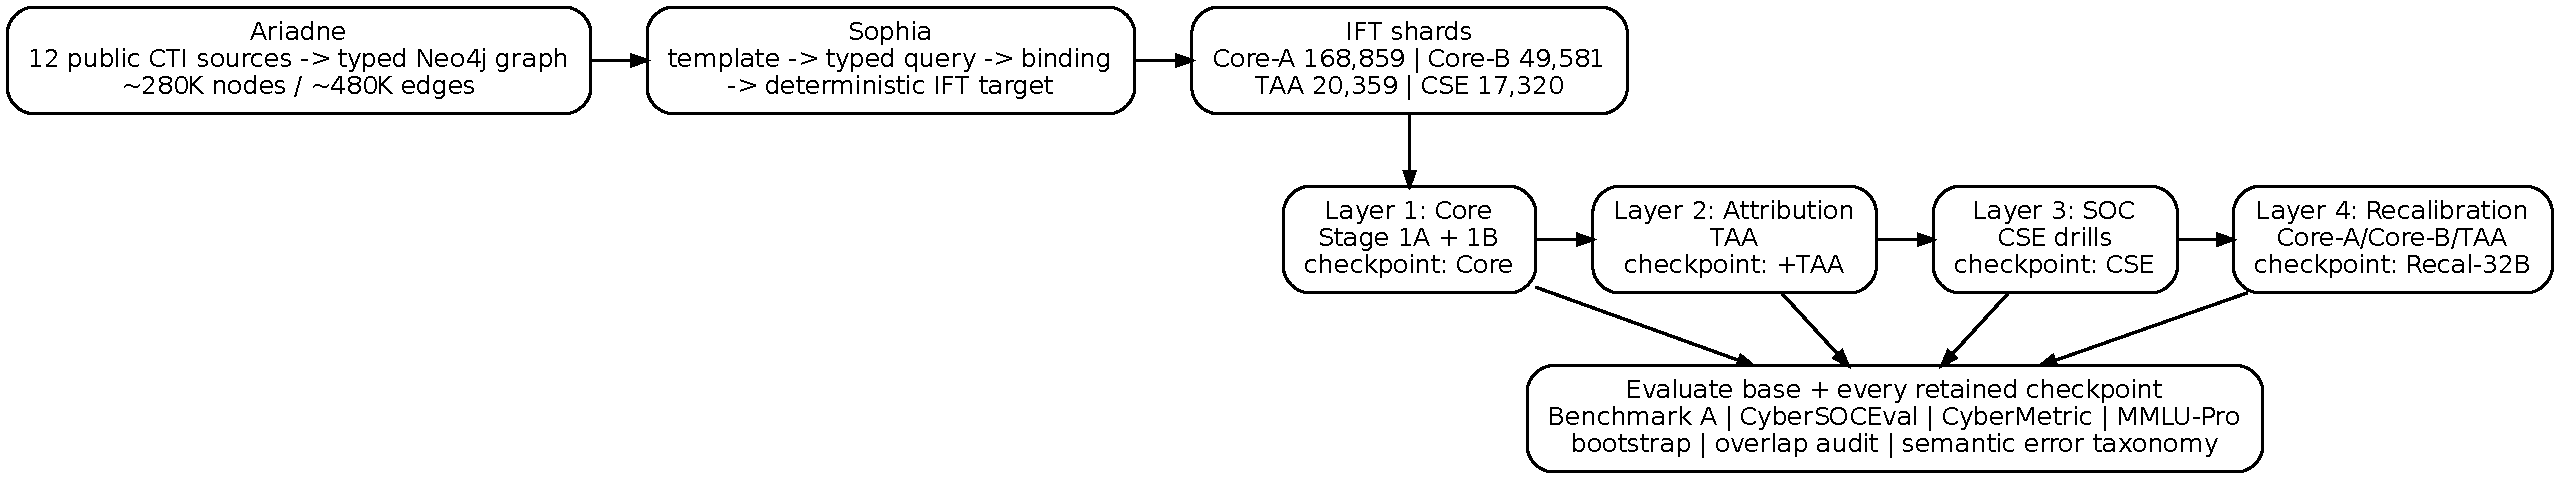
\includegraphics[width=0.98\textwidth]{figures/pipeline_greek_blind.pdf}
    \caption{Data and training pipeline. Ariadne integrates twelve public CTI sources into a versioned typed graph. Sophia executes typed queries and deterministically materializes IFT targets. The resulting shards feed four IFT layers whose checkpoints are retained for evaluation. The Ariadne and Sophia module names are preserved in the blind manuscript; author, institution, repository identity, and self-identifying benchmark citation details remain masked.}
    \label{fig:pipeline}
\end{figure*}

\subsection{Corpus Scope, Build Boundaries, and Artifactability}
The reported release uses four production CTI shards and three validation shards holding out 50 rows per template family. The Core corpus contained 219,675 rows after balancing. The 13-gram screen removed 684 rows, 550 were held out for validation, and the remaining records were split into Core-A (168,859) and Core-B (49,581), with a one-row accounting ambiguity in the phase-split report. The TAA and CSE shards contain 20,359 and 17,320 training rows, respectively. Core-A is trained with a general-purpose instruction mixture drawn from T\"ulu-3 SFT~\cite{lambert2024tulu} and Alpaca~\cite{taori2023alpaca}; these auxiliary examples are not Sophia-generated and were not included in the project-specific contamination screen.

Exact row-level regeneration was not fully seed-pinned in the audited release: graph-read order, sampling, and deduplication tie-breaks can vary. A reproducible release should retain hashes of serialized shards, source snapshots, counts after each filter, template versions, software versions, and random seeds. Source-relative auditability is therefore weaker than byte-identical repeatability unless the graph snapshot and generated corpus are preserved together.

Table~\ref{tab:boundaries} separates the assurances offered by each pipeline component. The code repository contains the Ariadne ingestion logic, Sophia templates and materializer, training launchers, evaluation harness, cost aggregator, and analysis scripts; it is referenced through the anonymized artifact entry~\cite{anonartifact}. The repository name and URL are intentionally withheld from the manuscript during review, while the artifact citation makes clear that executable code and supporting analysis exist independently of the prose.

\begin{table*}[t]
\caption{Pipeline boundaries and scope of assurance.}
\label{tab:boundaries}
\centering
\scriptsize
\setlength{\tabcolsep}{4pt}
\begin{tabular}{@{}p{0.13\textwidth}p{0.27\textwidth}p{0.24\textwidth}p{0.29\textwidth}@{}}
\toprule
Component & Input and transformation & Resulting artifact & Scope of assurance \\
\midrule
Ariadne & Public CTI records normalized to typed entities and relations & Versioned Neo4j CTI snapshot & Source-linked facts; not proof of completeness or correctness \\
Sophia & Expert-authored template, typed query, graph binding, deterministic rendering & Instruction, context, target, template identifier, source tags & Target traceable to executed graph binding \\
Corpus preparation & Generation, balancing, 13-gram screen, license gate, validation holdout, phase split & Core-A, Core-B, TAA, CSE, validation shards & Dependent on covered files, fields, thresholds, and retained build reports \\
Layered IFT & Layer-specific shard mixture and optimizer configuration & Core, +TAA, CSE, Recal-32B checkpoints & Observable transitions; no isolated causal effect of ordering \\
Evaluation & Fixed inputs, checkpoint, parser/scorer, serving settings & Predictions, per-item scores, run manifests & Reproducible to the extent complete run artifacts are retained \\
\bottomrule
\end{tabular}
\end{table*}

\section{Layered Instruction Fine-Tuning}
\subsection{Canonical 32B Configuration}
The canonical base is Qwen2.5-32B-Instruct~\cite{qwen25}. Training uses LlamaFactory~\cite{zheng2024llamafactory} with DeepSpeed ZeRO-3~\cite{rajbhandari2020zero}; the configured run additionally enables CPU offload, an 8-bit AdamW optimizer, gradient checkpointing, Liger kernels, and bfloat16 precision on eight 80-GB H100 GPUs. Effective batch size is preserved through gradient accumulation.

Table~\ref{tab:train} reports the schedule read from the release launchers. Layer 1 has two phases: Stage 1A mixes broad Core-A CTI families with auxiliary general instructions, and Stage 1B targets the RMS, ATE, VSP, and RCM schemas in Core-B. Layer 2 specializes threat-actor attribution with TAA records. Layer 3 uses CSE SOC-style structured-response drills. Layer 4 revisits earlier shards with a weighted mixture intended to rebalance the checkpoint. These are intended objectives; whether they are achieved is measured empirically rather than assumed from the schedule.

\begin{table*}[t]
\caption{Canonical Qwen2.5-32B layered IFT schedule. Caps are per-dataset maximum sample counts, not realized token counts. Wall-time budgets are documented planning figures for eight H100 GPUs.}
\label{tab:train}
\centering
\scriptsize
\setlength{\tabcolsep}{3.2pt}
\begin{tabular}{@{}llllllll@{}}
\toprule
Pass & Layer / input & Cap & Max tokens & Learning rate & Eff. batch & Packing & Budget (h) \\
\midrule
1A & Core-A + T\"ulu-3 SFT + Alpaca & 240,000/dataset & 8,192 & $1\times10^{-5}$ & 16 & on & 26--30 \\
1B & Core-B & 70,000 & 16,384 & $5\times10^{-6}$ & 8 & off & included \\
2 & TAA & 33,000 & 4,096 & $5\times10^{-6}$ & 16 & on & 13--17 \\
3 & CSE & 33,000 & 4,096 & $5\times10^{-6}$ & 16 & on & 9--13 \\
4 & Core-A/Core-B/TAA, 0.15/0.60/0.25 & 3,600/shard & 16,384 & $3\times10^{-6}$ & 8 & off & 3--4 \\
\bottomrule
\end{tabular}
\end{table*}

The caps exceed the realized Core-B, TAA, and CSE shard sizes, so those passes consume their shards in one epoch. In Stage 1A the cap applies independently to the Sophia shard and each auxiliary dataset, so the general mixture can contribute up to 240,000 rows alongside 168,859 Core-A rows; its contribution is therefore material to the forgetting discussion. Layer 4 interleaves the three listed shards under the stated probabilities and per-shard cap, yielding about 6,000 sampled examples. Neither repeated exposure nor actual token consumption can be inferred from maximum sequence length and sample caps alone.

The alternative Layer-4 recipe used by the 14B port employs learning rate $10^{-6}$, mixture probabilities 0.25/0.40/0.35, and a 2,400-example cap. Both Stage-4 recipes were also trained from the same CSE parent on the 32B chain for direct comparison. Because some ports use different final-layer settings and the Qwen3 port changes serving mode, cross-architecture results are transfer evidence rather than a clean model-size ablation.

\section{Evaluation Protocol}
\subsection{Task Portfolio, Scorers, and Run Records}
Benchmark A contains CTI knowledge (CKT), attack-technique extraction (ATE), root-cause mapping (RCM), risk-mitigation strategy (RMS), vulnerability-severity prediction (VSP), and threat-actor attribution (TAA) in Classic and Canonical forms. CyberSOCEval supplies malware-analysis and threat-intelligence-reasoning tasks~\cite{deason2025cybersoceval}; CyberMetric supplies 2K and 10K cybersecurity multiple-choice tiers~\cite{tihanyi2024cybermetric}; and MMLU-Pro is used as a separate general-task diagnostic~\cite{wang2024mmlupro}.

\begin{table}[t]
\caption{Evaluation portfolio for the canonical chain.}
\label{tab:eval}
\centering
\scriptsize
\setlength{\tabcolsep}{3.2pt}
\begin{tabular}{@{}lrl@{}}
\toprule
Task & Items & Per-item score \\
\midrule
CKT & 3,000 & exact option \\
RCM & 2,000 & exact CWE \\
VSP & 2,000 & normalized CVSS distance \\
ATE & 500 & parent-technique match \\
RMS & 500 & mitigation set F1 \\
TAA Classic & 100 & exact / related group \\
TAA Canonical & 133 & canonical/G-code or alias \\
CyberSOCEval & 609/588 & strict + Jaccard \\
CyberMetric & 2,000/10,180 & exact option \\
MMLU-Pro & 12,032 & exact option \\
\bottomrule
\end{tabular}
\end{table}

CKT, RCM, CyberMetric, and MMLU-Pro use exact option or identifier matching. ATE grants credit at the parent-technique level. VSP parses CVSS v3.1 vectors and derives their standard base scores according to the FIRST specification~\cite{first2019cvss}; the retained project scorer then applies the normalized distance $1-|s_{pred}-s_{gold}|/7.7$. Two of 2,000 vectors at the final checkpoint are unparseable and excluded by that scorer. RMS uses set F1, with the reported combined variant assigning half credit to mitigations in the target technique's neighborhood. TAA Classic awards full credit to an alias-connected group, half credit to a related group, and zero otherwise. TAA Canonical awards full credit for the canonical name or G-code and half credit for another recognized alias. CyberSOCEval scores answer-letter sets with both strict accuracy and Jaccard similarity. These metrics differ in kind and should not all be called accuracy or interpreted as calibrated operational probabilities.

Local checkpoints were served with vLLM~\cite{kwon2023vllm} on two H100 GPUs at batch size 32 (64 for MMLU-Pro). Each score is a single evaluation of a single training run. Per-item predictions and score files were retained for the five fine-tuned checkpoints and are the basis of the bootstrap and error analyses. Corresponding item-level files for the base and hosted references were unavailable for the audit, so paired statistics involving those rows are not reported.

\subsection{Alignment Between Training and Evaluation}
Alignment is deliberate. Core-B trains the schemas assessed by Benchmark-A mapping and mitigation tasks; the TAA layer targets attribution; CSE targets SOC-style answer formats; and Core-A includes multiple-choice and CyberMetric-like families. None of the CTI benchmark families is a demonstrably untouched target. Sharing public catalogs is appropriate when the objective is catalog competence, but independent data-generation pipelines do not establish entity-disjoint, fact-disjoint, or temporally held-out evaluation. The results must therefore distinguish schema adaptation from stronger claims about unseen facts and enterprise incidents.

\subsection{Aggregation and Item-Level Uncertainty}
To avoid hiding Canonical-TAA behavior, we define the balanced attribution score and two aggregates:
\begin{equation}
T_{bal}=\tfrac{1}{2}(T_{Classic}+T_{Canonical}),
\end{equation}
\begin{equation}
A_{bal}=\tfrac{1}{6}(K+E+R+M+V+T_{bal}),
\end{equation}
\begin{equation}
B_{bal}=\tfrac{1}{3}(A_{bal}+C+Y),
\end{equation}
where $K,E,R,M,V$ denote CKT, ATE, RCM, combined RMS, and VSP; $Y$ is the mean of the CyberMetric tiers; and $C$ is the retained CyberSOCEval composite, namely the mean of malware strict accuracy, malware Jaccard, and threat-intelligence strict accuracy. The asymmetric CyberSOCEval convention is retained because it is the rule used by the audited results workbook for every model row; a symmetric four-metric mean does not materially change the base-to-final conclusion.

For the five fine-tuned checkpoints, 95\% percentile bootstrap intervals are computed with 2,000 item-resampling replicates, following the standard nonparametric bootstrap framework~\cite{efron1993bootstrap}. Differences between checkpoints use the same resampled items for both members of a pair, producing paired item-level estimates. These intervals quantify item-sampling uncertainty for fixed trained checkpoints; they do not measure training-seed variance. Clustered questions from a common source are also treated as independent, making the intervals somewhat optimistic where benchmark items are correlated.

\section{Contamination and Training-Evaluation Overlap}
\subsection{Verbatim 13-Gram Screening}
Before training, each project-generated shard was scanned for verbatim overlap with locally available evaluation files. The filter lowercases alphanumeric tokens and indexes distinct 13-word sequences, following the scale used in the GPT-3 contamination audit~\cite{brown2020language}. A single shared 13-gram flags a row for audit; at least 50 shared sequences with one indexed evaluation record trigger removal. Table~\ref{tab:contam} reports the retained build statistics.

\begin{table*}[t]
\caption{Verbatim 13-gram screen. ``Flagged'' rows share at least one 13-gram with an indexed evaluation record; rows at 50 or more shared 13-grams were removed.}
\label{tab:contam}
\centering
\scriptsize
\setlength{\tabcolsep}{3.0pt}
\begin{tabular}{@{}lrrrrrrrrr@{}}
\toprule
Shard & Scanned & 1 & 2--4 & 5--12 & 13--24 & 25--49 & $\geq$50 removed & Flagged total & Retained \\
\midrule
Core & 219,675 & 6,641 & 10,952 & 6,656 & 3,165 & 6,799 & 684 & 34,897 (15.9\%) & 218,991 \\
TAA & 20,509 & 0 & 0 & 0 & 0 & 0 & 0 & 0 & 20,509 \\
CSE & 17,670 & 24 & 17 & 0 & 0 & 0 & 0 & 41 (0.2\%) & 17,670 \\
\bottomrule
\end{tabular}
\end{table*}

The screen has important coverage limits. CyberSOCEval question files were fetched into the evaluation directory at run time and were not present when the shards were built, so CSE was screened only against the files available at build time. The auxiliary T\"ulu-3 and Alpaca mixtures were not screened, and base-model pretraining contamination is outside scope. Index keys use file basenames and row indices, selected text fields are extracted, and the 50-overlap threshold cannot remove a complete duplicate shorter than 62 tokens because such a record contains fewer than 50 distinct 13-grams. We therefore describe the procedure as a measured verbatim-overlap screen rather than calling the corpus fully decontaminated. Stronger practice would add hash-based exact deduplication, full-path identifiers, and complete screening of every evaluation source. Open efforts such as OLMo provide a useful comparison because they release training data together with training and evaluation code, making the data pipeline directly inspectable~\cite{groeneveld2024olmo}.

\subsection{Entity and Gold-Fact Overlap}
Verbatim screening misses a more relevant case for graph-generated supervision: a training row can state the evaluated fact using different wording. We therefore measured whether an evaluation item's identifying entity and complete gold answer co-occur in one training row. Table~\ref{tab:overlap} reports the resulting overlap and the final checkpoint's subset score.

\begin{table*}[t]
\caption{Training overlap with Benchmark-A items. ``Gold fact in one row'' means that the identifying entity and complete gold answer co-occur in a single training row.}
\label{tab:overlap}
\centering
\scriptsize
\setlength{\tabcolsep}{3.5pt}
\begin{tabular}{@{}lrrrrr@{}}
\toprule
Task & Items & Entity in training & Gold fact in one row & Final: fact present & Final: fact absent \\
\midrule
RCM & 2,000 & 660 (33.0\%) & 137 (6.9\%) & 66.4 ($n=137$) & 64.3 ($n=1,340$) \\
VSP & 2,000 & 446 (22.3\%) & 7 (0.4\%) & 77.4 ($n=445$) & 77.9 ($n=1,553$) \\
ATE & 500 & 500 (100\%) & n/a & 70.5 (top exposure tertile) & 62.3 (bottom tertile) \\
RMS & 500 & 500 (100\%) & 273 (54.6\%) & 53.8 ($n=273$) & 73.1 ($n=227$) \\
TAA Canonical & 133 & 40 aliases (30.1\%) & 38 (28.6\%) & 7.9 ($n=38$) & 1.6 ($n=93$) \\
\bottomrule
\end{tabular}
\end{table*}

The subset scores do not show the pattern expected from simple memorization of leaked test items. RCM items whose exact CVE-to-CWE pair appears in training score within about two points of items whose CVE never appears. VSP is effectively unchanged between CVEs present and absent from training. RMS is lower when the entire mitigation set is present because those techniques tend to have larger mitigation sets on which set F1 is more difficult. Two tasks do track exposure: ATE accuracy rises with the frequency of the gold technique, and at the +TAA checkpoint Canonical-TAA items whose alias-to-group mapping occurs in training score 52.6 against 30.6 for the remainder. These patterns are consistent with catalog competence, but semantic paraphrases, repeated public facts, and benchmark-guided recipe selection remain uncontrolled. An entity-disjoint or temporally held-out incident set is still required for a strong out-of-sample claim.

\section{Results}
\subsection{Canonical 32B Chain}
Table~\ref{tab:mainresults} reports the base model and the retained checkpoints. The final checkpoint raises ATE from 18.2 to 65.8, RMS from 7.6 to 62.5, CKT from 52.9 to 75.5, and RCM from 59.5 to 67.1. VSP decreases by 1.0 point and MMLU-Pro by 11.6. The balanced Benchmark-A score rises from 40.3 to 62.6 and the three-benchmark mean from 57.7 to 65.0. The item-bootstrap interval for the final $B_{bal}$ is 64.1--66.0 and for $A_{bal}$ is 61.5--63.7.

\begin{table*}[t]
\caption{Task scores and aggregates for the canonical Qwen2.5-32B chain (0--100; one evaluation per checkpoint). TAA is shown as Classic/Canonical.}
\label{tab:mainresults}
\centering
\scriptsize
\setlength{\tabcolsep}{3.0pt}
\begin{tabular}{@{}lrrrrrrrrrrr@{}}
\toprule
Checkpoint & CKT & ATE & RCM & RMS & VSP & TAA C/Can & $C$ & $Y$ & MMLU-Pro & $A_{bal}$ & $B_{bal}$ \\
\midrule
Base & 52.9 & 18.2 & 59.5 & 7.6 & 78.8 & 48.0/2.0 & 42.6 & 90.2 & 69.0 & 40.3 & 57.7 \\
Core & 72.9 & 67.2 & 69.8 & 63.8 & 83.1 & 46.5/18.4 & 31.1 & 89.6 & 59.2 & 64.9 & 61.9 \\
+TAA & 75.4 & 63.4 & 69.0 & 62.9 & 83.5 & 47.0/36.8 & 29.8 & 89.4 & 58.2 & 66.0 & 61.7 \\
CSE & 72.5 & 63.4 & 67.7 & 63.7 & 78.9 & 53.5/3.4 & 42.0 & 88.8 & 54.2 & 62.4 & 64.4 \\
Recal-32B & 75.5 & 65.8 & 67.1 & 62.5 & 77.8 & 50.5/3.4 & 42.6 & 89.8 & 57.4 & 62.6 & 65.0 \\
\bottomrule
\end{tabular}
\end{table*}

The cross-benchmark improvement is not uniform. Benchmark A contributes approximately +7.4 points to the 7.3-point change in $B_{bal}$, while CyberSOCEval remains 42.6 and CyberMetric moves from 90.2 to 89.8. The positive contribution therefore comes from the benchmark that the training shards target most directly. This is evidence of schema adaptation, not uniform transfer across independently targeted CTI workloads.

\subsection{Layer Transitions and Paired Intervals}
The retained checkpoints reveal where capabilities move. The TAA layer raises Canonical attribution from 18.4 to 36.8, a paired change of +18.4 points with 95\% interval [12.4, 24.4], and raises CKT by +2.6 [1.0, 4.2]. Most other changes are small; MMLU-Pro decreases by 1.0 [-1.7, -0.4]. Under the balanced aggregation, Benchmark A peaks at +TAA, whereas $B_{bal}$ changes by only -0.1 [-0.6, 0.4].

The CSE layer produces the clearest interference. Relative to +TAA, CyberSOCEval malware strict accuracy rises by 19.7 [15.3, 24.2] and threat-intelligence strict accuracy by 7.9 [3.3, 12.4], but Canonical TAA falls by 33.5 [-39.8, -27.1], VSP by 4.5 [-5.5, -3.5], CKT by 3.0 [-4.5, -1.4], and MMLU-Pro by 4.0 [-4.8, -3.2]. The final recalibration recovers CKT, CyberSOCEval threat-intelligence accuracy, CyberMetric 10K, and MMLU-Pro, but it does not restore Canonical TAA and leaves VSP below both its CSE parent and the base.

\begin{table*}[t]
\caption{Paired checkpoint differences (later minus earlier) with 95\% item-bootstrap intervals. Asterisks indicate intervals excluding zero.}
\label{tab:transitions}
\centering
\scriptsize
\setlength{\tabcolsep}{2.5pt}
\begin{tabular}{@{}lrrrr@{}}
\toprule
Metric & +TAA $-$ Core & CSE $-$ +TAA & Recal-32B $-$ CSE & Recal-32B $-$ Core \\
\midrule
CKT & +2.6 [1.0,4.2]* & -3.0 [-4.5,-1.4]* & +3.1 [1.5,4.6]* & +2.7 [1.1,4.2]* \\
ATE & -3.8 [-7.6,0.2] & 0.0 [-4.8,4.6] & +2.4 [-2.4,7.2] & -1.4 [-5.2,2.8] \\
RCM & -0.8 [-1.3,-0.2]* & -1.3 [-2.2,-0.4]* & -0.6 [-1.9,0.8] & -2.7 [-3.9,-1.5]* \\
RMS & -1.0 [-3.3,1.6] & +0.9 [-1.5,3.3] & -1.2 [-3.9,1.5] & -1.3 [-4.0,1.4] \\
VSP & +0.3 [-0.1,0.7] & -4.5 [-5.5,-3.5]* & -1.1 [-2.3,0.0] & -5.3 [-6.4,-4.2]* \\
TAA Canon. & +18.4 [12.4,24.4]* & -33.5 [-39.8,-27.1]* & 0.0 [-3.0,2.6] & -15.0 [-20.7,-9.4]* \\
CSE malware & +0.6 [-0.4,1.6] & +19.7 [15.3,24.2]* & -1.8 [-4.5,1.0] & +18.6 [14.9,22.5]* \\
CSE threat intel & -4.5 [-6.7,-2.3]* & +7.9 [3.3,12.4]* & +4.4 [1.8,7.2]* & +7.9 [3.6,12.0]* \\
MMLU-Pro & -1.0 [-1.7,-0.4]* & -4.0 [-4.8,-3.2]* & +3.2 [2.5,3.9]* & -1.8 [-2.6,-1.1]* \\
$A_{bal}$ & +1.1 [0.1,2.2]* & -3.6 [-4.8,-2.3]* & +0.2 [-0.9,1.3] & -2.3 [-3.4,-1.1]* \\
$B_{bal}$ & -0.1 [-0.6,0.4] & +2.7 [1.7,3.8]* & +0.6 [-0.2,1.4] & +3.2 [2.2,4.2]* \\
\bottomrule
\end{tabular}
\end{table*}

These comparisons are diagnostic rather than causal ablations. Core$\rightarrow$CSE without the TAA layer and a one-stage mixture with matched realized tokens and updates were not run. Repeated seeds under a frozen selection rule are also required to distinguish a robust recipe effect from training stochasticity. The label ``final'' denotes the released checkpoint, not a statistically established global optimum.

\subsection{Why Canonical Attribution Collapses}
Aggregate scores cannot distinguish a loss of attribution knowledge from a formatting change, so every Canonical-TAA response of the five retained checkpoints was classified. Table~\ref{tab:taaerrors} shows that the collapse is semantic. At CSE, every response is well formed and 124 of 133 name a real ATT\&CK group that is nevertheless the wrong one; the model also stops emitting G-codes entirely. At +TAA, 64 responses name another recognized alias of the correct group and therefore receive half credit. Classic TAA has a different profile, with a large fraction of responses receiving plausibility credit for related groups rather than exact attribution.

\begin{table}[t]
\caption{Canonical-TAA response taxonomy (133 items).}
\label{tab:taaerrors}
\centering
\scriptsize
\setlength{\tabcolsep}{2.7pt}
\begin{tabular}{@{}lrrr@{}}
\toprule
Outcome & +TAA & CSE & Recal-32B \\
\midrule
Strict correct & 17 & 4 & 3 \\
Correct alias & 64 & 1 & 3 \\
Wrong known group & 32 & 124 & 113 \\
Other/missing & 20 & 4 & 14 \\
Contains G-code & 132 & 0 & 121 \\
\bottomrule
\end{tabular}
\end{table}

The result matters because a parser-only diagnosis would imply that the underlying association knowledge remains available but is merely serialized differently. Instead, CSE mostly produces plausible, well-formed, incorrect group names. The SOC-oriented layer therefore appears to overwrite or redirect the association behavior itself. Recalibration restores G-code formatting but not correctness, providing a concrete example of why retained intermediate checkpoints reveal more than a final aggregate score.

\subsection{Where Severity Prediction Regresses}
VSP is scored by CVSS base-score distance, so a checkpoint can score 77.8 while exactly matching all eight base metrics in only 13.6\% of items. Table~\ref{tab:vsp} decomposes the errors. Exact-vector agreement falls from 25.6\% at +TAA to 16.4\% at CSE and 13.6\% at Recal-32B. The regression concentrates in exploitability fields: Attack Vector mismatches increase from 136 to 537 at CSE and 583 at Recal-32B; Privileges Required from 357 to 799 and 791; Scope from 115 to 421 and 525. Impact metrics are comparatively stable. The CSE layer thus shifts the model's judgment of how a vulnerability is reached more than what it affects, a behavior partly hidden by the scalar base-score metric.

\begin{table}[t]
\caption{VSP error profile over 2,000 items. Columns after ``Exact'' are counts of items mismatching each CVSS v3.1 base metric.}
\label{tab:vsp}
\centering
\scriptsize
\setlength{\tabcolsep}{2.2pt}
\begin{tabular}{@{}lrrrrrrrrr@{}}
\toprule
Checkpoint & Exact & AV & AC & PR & UI & S & C & I & A \\
\midrule
Core & 483 & 149 & 127 & 369 & 344 & 163 & 634 & 653 & 341 \\
+TAA & 513 & 136 & 131 & 357 & 342 & 115 & 618 & 661 & 340 \\
CSE & 329 & 537 & 125 & 799 & 422 & 421 & 578 & 504 & 356 \\
Recal-32B & 271 & 583 & 211 & 791 & 372 & 525 & 601 & 507 & 444 \\
\bottomrule
\end{tabular}
\end{table}

\subsection{Qualitative Schema Examples}
Three retained examples illustrate how errors change between Core and the final checkpoint; they are illustrative rather than a representative error sample. For an ATE item describing stolen SSH credentials used to log into a Linux build server, Core answers T1078 (Valid Accounts) and the final checkpoint answers T1021.004 (Remote Services: SSH), which the parent-level scorer credits against the gold technique. For an RCM item describing local unauthenticated file tampering in a SCADA product, the answer changes from CWE-732 to the gold CWE-276 (Incorrect Default Permissions). For a CKT item about a mobile malware audio-capture capability, the answer changes from the wrong option to the gold ATT\&CK technique. These examples demonstrate schema correction, while the aggregate and overlap analyses determine whether the behavior is systematic.

\subsection{Transfer Across Model Families}
Table~\ref{tab:ports} reports the selected checkpoint of each port under the uniform aggregation. The dense Qwen ports gain on every CTI aggregate while losing 11.6--13.9 MMLU-Pro points. The sparse Qwen3 port gains 1.6 points on $B_{bal}$ and 6.0 on the ten-test mean but loses 24.6 MMLU-Pro points; its base was evaluated with thinking mode enabled while the fine-tuned checkpoints were served without it, so the comparison mixes a serving change with the training effect. The two 8B ports are negative under $B_{bal}$ despite some gains on the CTI test mean. Applying the same layered recipe to an already security-specialized or much smaller base is therefore not recommended without architecture-specific tuning.

\begin{table*}[t]
\caption{Cross-architecture ports under the uniform aggregation. Values compare each base to the project's selected checkpoint; all rows are single training/evaluation runs.}
\label{tab:ports}
\centering
\scriptsize
\setlength{\tabcolsep}{3.3pt}
\begin{tabular}{@{}llrrrrrrrrr@{}}
\toprule
& & \multicolumn{3}{c}{$B_{bal}$} & \multicolumn{3}{c}{Ten-test mean} & \multicolumn{3}{c}{MMLU-Pro} \\
Base model & Selected checkpoint & Base & Port & $\Delta$ & Base & Port & $\Delta$ & Base & Port & $\Delta$ \\
\midrule
Qwen2.5-32B-Instruct & Recal-32B & 57.7 & 65.0 & +7.3 & 49.6 & 62.9 & +13.3 & 69.0 & 57.4 & -11.6 \\
Qwen2.5-14B-Instruct & Recalibrate & 55.1 & 61.0 & +5.9 & 46.1 & 59.6 & +13.5 & 64.1 & 50.2 & -13.9 \\
Qwen3-30B-A3B-Thinking & CSE & 61.8 & 63.4 & +1.6 & 54.9 & 60.9 & +6.0 & 77.6 & 53.0 & -24.6 \\
Foundation-Sec-8B-Instruct & Recalibrate & 56.4 & 53.5 & -2.9 & 52.7 & 53.2 & +0.4 & 43.2 & 25.6 & -17.6 \\
Llama-3.1-8B-Instruct & Recalibrate & 50.7 & 49.8 & -0.9 & 43.4 & 50.8 & +7.3 & 48.3 & 27.7 & -20.6 \\
\bottomrule
\end{tabular}
\end{table*}

\subsection{Hosted Reference Models}
The final 32B checkpoint was also placed against hosted reference models evaluated with the same harness. Table~\ref{tab:hosted} uses the same balanced attribution convention for every row. The purpose is contextual rather than a claim of direct product equivalence: hosted systems differ in scale, training data, reasoning settings, serving constraints, and cost. The local checkpoint remains below the strongest hosted systems on the three-benchmark aggregate and substantially below them on MMLU-Pro, while its Benchmark-A score is comparatively closer. This reinforces the interpretation that the layered IFT recipe produces narrow CTI specialization rather than broad capability parity.

\begin{table*}[t]
\caption{Hosted references and the local 32B models under the uniform aggregation (single evaluations). $C$ is the CyberSOCEval composite and $Y$ the CyberMetric mean.}
\label{tab:hosted}
\centering
\scriptsize
\setlength{\tabcolsep}{4.0pt}
\begin{tabular}{@{}lrrrrrr@{}}
\toprule
Model & $A_{bal}$ & $C$ & $Y$ & $B_{bal}$ & Ten-test mean & MMLU-Pro \\
\midrule
GPT-5.5 & 77.0 & 48.3 & 93.3 & 72.9 & 73.5 & 88.3 \\
DeepSeek-V4-Pro & 67.2 & 52.2 & 91.8 & 70.4 & 67.9 & 79.1 \\
Gemini-3-Flash-Preview & 69.3 & 48.1 & 92.1 & 69.8 & 68.4 & 89.2 \\
GPT-5.2 & 63.8 & 46.8 & 91.9 & 67.5 & 65.0 & 81.3 \\
DeepSeek-V3.2-Exp & 59.0 & 47.2 & 91.7 & 66.0 & 62.2 & 82.5 \\
Local Recal-32B & 62.6 & 42.6 & 89.8 & 65.0 & 62.9 & 57.4 \\
Gemini-2.5-Flash & 53.1 & 46.2 & 91.1 & 63.4 & 57.9 & 82.1 \\
Qwen2.5-32B-Instruct base & 40.3 & 42.6 & 90.2 & 57.7 & 49.6 & 69.0 \\
\bottomrule
\end{tabular}
\end{table*}

The local model is 7.9 points below GPT-5.5, 5.4 below DeepSeek-V4-Pro, 4.8 below Gemini-3-Flash-Preview, 2.5 below GPT-5.2, and 1.0 below DeepSeek-V3.2-Exp on $B_{bal}$, while exceeding Gemini-2.5-Flash by 1.6 points. On the ten-test CTI mean it lies between GPT-5.2 and DeepSeek-V3.2-Exp. Its MMLU-Pro score is 20--30 points below the hosted references. These rows are single runs and the hosted manifests were not re-audited at the same level as the retained local checkpoints, so the comparison should be read as a reference frame rather than a controlled statistical ranking.

\section{Evaluation Expenditure and Artifact Scope}
The project cost ledger combines hosted-API token accounting with local elapsed-time accounting at an assumed \$2.50 per GPU-hour on a two-H100 host. The audit found that the local aggregator counted a model-level summary in addition to the underlying task summaries, exactly doubling every local row. Recomputing the five retained 32B checkpoints from the run manifests gives single-pass totals of \$1.44 for Core, \$1.36 for +TAA, \$1.09 for CSE, \$1.25 for the alternative recalibration, and \$1.42 for Recal-32B. The final checkpoint's three CTI benchmark families account for about \$1.02 of its \$1.42 total; MMLU-Pro accounts for about \$0.39.

\begin{table*}[t]
\caption{Recorded evaluation expenditure in USD. Hosted rows are API token ledgers and may include reruns. Local rows marked ``run record'' are single passes recomputed from per-suite manifests on two H100 GPUs at the assumed $\$2.50$ per GPU-hour rate. No training cost is included.}
\label{tab:cost}
\centering
\scriptsize
\setlength{\tabcolsep}{3.8pt}
\begin{tabular}{@{}lrrrrrl@{}}
\toprule
Model & Benchmark A & CyberSOCEval & CyberMetric & MMLU-Pro & CTI-only & Total / basis \\
\midrule
GPT-5.5 & 202.62 & 79.19 & 38.73 & 187.60 & 320.53 & 508.13 / API ledger \\
GPT-5.2 & 30.44 & 23.28 & 4.04 & 151.90 & 57.77 & 209.67 / API ledger \\
DeepSeek-V4-Pro & 0.32 & 27.93 & 9.87 & 88.28 & 38.12 & 126.40 / API ledger \\
DeepSeek-V3.2-Exp & 0.01 & 3.68 & 0.45 & 7.10 & 4.14 & 11.24 / API ledger \\
Core & 0.53 & 0.33 & 0.12 & 0.47 & 0.98 & 1.44 / run record \\
+TAA & 0.49 & 0.33 & 0.11 & 0.43 & 0.93 & 1.36 / run record \\
CSE & 0.37 & 0.29 & 0.11 & 0.31 & 0.77 & 1.09 / run record \\
Recal-32B & 0.61 & 0.30 & 0.12 & 0.39 & 1.02 & 1.42 / run record \\
\bottomrule
\end{tabular}
\end{table*}

For a fixed workload definition and acceptable quality level, a useful lifecycle framing separates fixed specialization cost from per-workload inference cost. Let
\begin{equation}
C_{train}=\sum_s g_s h_s r_s,
\end{equation}
where $g_s$ is GPU count, $h_s$ elapsed training hours, and $r_s$ cost per GPU-hour for layer $s$. If $C_{fixed}$ additionally includes graph construction, corpus generation, and setup, then for $N$ comparable workloads one can write $C_{local}(N)=C_{fixed}+C_{maint}(N)+Nc_L$ and $C_{API}(N)=Nc_A$. Ignoring maintenance or absorbing it into $C_{fixed}$, the first break-even workload count is
\begin{equation}
N_{BE}=\left\lceil\frac{C_{fixed}}{c_A-c_L}\right\rceil,\qquad c_A>c_L,
\end{equation}
with no finite break-even when $c_A\le c_L$. The equation, rather than any one point estimate, is the defensible result because model quality, token generation behavior, provider pricing, utilization, and refresh costs all vary.

The training plan documents 51--64 wall-clock hours on eight H100 GPUs, equivalent to 408--512 GPU-hours or approximately \$1,020--\$1,280 at the same assumed rate for one successful chain. This is a planning figure, not a metered lifecycle cost, and excludes data construction, failed experiments, standing capacity, engineering labor, maintenance, refresh training, electricity, and depreciation. Likewise, hosted API ledgers may include reruns and models differ in capability and response length. The economic evidence is therefore useful for experimental accounting but not for a claim that a local SLM has a universal production cost advantage.

For reproducibility, the anonymized software artifact~\cite{anonartifact} is intended to provide the code path that connects the paper's claims to executable components: Ariadne ingestion, Sophia template parsing/materialization, corpus preparation, layer-specific launchers, evaluation parsers/scorers, and the analysis scripts used for overlap, bootstrap, error-taxonomy, and cost recomputation. The manuscript deliberately does not print a repository URL or institutional namespace because either could reveal author identity. The camera-ready version can restore the public repository name, commit, and checkpoint links after double-blind review.

\section{Discussion: Implications for Cybersecurity SLM Design}
The results suggest that graph-grounded template generation and layered IFT address different failure surfaces and should be evaluated separately. Ariadne and Sophia operate on the supervision side: they make the origin of a target inspectable and allow coverage to be designed around explicit CTI schemas. The retained checkpoints operate on the optimization side: they reveal how later specialization changes behavior that earlier layers had already acquired. Conflating the two would overstate what the experiment shows. The graph path is directly auditable; the superiority of the four-layer order is not yet established.

For SLM-oriented systems, the distinction is especially useful because limited model capacity and aggressive specialization create a practical tension between narrow competence and retained general capability. The 32B chain gains strongly on schema-aligned tasks while losing MMLU-Pro, and the 8B ports show that a recipe successful on a larger base can fail under the same aggregate. A deployment that treats an SLM as a compact general replacement for a frontier model would therefore miss the central trade-off exposed by the data. A more defensible architecture treats the SLM as a bounded specialist whose accepted task types are defined by measured competence, with broader reasoning routed elsewhere when needed.

The transition analysis also argues for retaining intermediate checkpoints rather than training only to a final release. The +TAA checkpoint is materially better at canonical attribution than the CSE and Recal-32B checkpoints, while CSE improves SOC-style tasks. This means a single linear sequence can move the model between different capability profiles rather than monotonically improving one universal objective. In practice, checkpoint retention supports at least three strategies: selecting the checkpoint whose profile matches a deployment role, routing different task families to different checkpoints, or using the observed regressions to construct replay mixtures and control experiments for the next training cycle. The present work evaluates the first strategy diagnostically but does not test multi-checkpoint routing.

Sophia's deterministic materialization is also relevant to SLM data efficiency. A bounded CTI schema can generate many instruction forms whose labels are tied to the same underlying graph facts, allowing the training corpus to emphasize coverage, normalization, and output discipline without relying on a second language model to invent the gold target. The study does not establish that this is more sample-efficient than an LLM-generated or expert-authored matched corpus, because such a control was not run. It does, however, reduce one important source of ambiguity: when a generated row is wrong relative to the intended graph semantics, the template, binding, and source path can be inspected directly.

\section{Threats to Validity and Operational Boundaries}
\textbf{Attribution of benefit.} Graph-derived data, shard composition, training duration, order, sequence length, packing, and hyperparameters co-vary. The retained checkpoints demonstrate observable transitions, not the superiority of graph-generated data over a matched alternative or the necessity of the four-layer schedule. A Core$\rightarrow$CSE skip-layer control and an equal-token mixed-data control are required for stronger causal claims.

\textbf{Evaluation alignment and selection.} The primary gain occurs on the benchmark most directly aligned with the training schemas. Exact gold-fact overlap does not explain the mapping gains, but public-catalog overlap, common answer spaces, unscreened auxiliary data, incomplete verbatim-screen coverage, and repeated benchmark-guided recipe development limit out-of-sample interpretation. Benchmark A also has contributor overlap with this study, which is why its identifying citation details are masked. A stronger extension would freeze an Ariadne snapshot, select checkpoints on separate development data, and evaluate once on a later independently constructed, entity-disjoint incident set.

\textbf{Uncertainty.} The bootstrap intervals cover item sampling for the specific trained checkpoints, not training-seed variance. Several independently seeded Layer-4 runs would test the narrow recipe-selection question; independently seeded replication of the full chain would be required for stronger layer-effect claims. No significance test beyond the paired intervals is asserted.

\textbf{Catalog competence versus operational safety.} The final Canonical-TAA score does not support autonomous actor attribution, and the VSP error profile shows systematic exploitability misjudgment after CSE. The 11.6-point MMLU-Pro decrease at 32B and larger losses on several ports motivate explicit workload boundaries. Prompt-injection resistance, private-telemetry performance, latency under concurrent load, secure autonomous tool use, and human-analyst utility were not established. The specialized model should not be the sole basis for high-consequence attribution, incident containment, unrestricted tool execution, legal advice, or decisions requiring broad reasoning outside validated CTI schemas.

\textbf{Auditability versus repeatability.} Source-relative auditability is distinct from exact replay. Replaying Sophia generation requires immutable Ariadne and template snapshots; reproducing training also requires the serialized rows, seeds, environment, and optimizer settings; reproducing evaluation requires complete inputs, outputs, scoring code, serving settings, and run boundaries. The retained artifacts satisfy more of this chain for the fine-tuned checkpoints than for the base model or hosted references.

\section{Conclusion}
This work combines Ariadne, a versioned graph of public CTI, with Sophia, a typed-query template engine, to make IFT target construction source-resolvable. On top of that graph-grounded data plane, a layered IFT schedule retains checkpoints after Core, threat-attribution, SOC-oriented, and recalibration phases. The canonical 32B chain produces large gains in attack-technique extraction, mitigation scoring, CTI knowledge, and root-cause mapping, raising the uniformly defined three-benchmark mean from 57.7 to 65.0.

The same checkpoint-level audit exposes material interference. Canonical attribution collapses after the CSE layer through wrong-but-well-formed group names rather than parser failure; VSP regressions concentrate in Attack Vector, Privileges Required, and Scope; and MMLU-Pro declines. Cross-architecture ports show that the recipe does not transfer uniformly to smaller or already specialized bases. The overlap analysis also shows why benchmark provenance must be treated as more than verbatim deduplication: public-catalog competence, exposure frequency, and exact fact overlap are distinct phenomena.

The evidence supports graph-grounded template generation, layered-checkpoint diagnosis, and explicit provenance boundaries. It does not yet establish that the four-layer schedule is necessary or superior, that gains extend to unseen enterprise incidents, or that experimental cost ratios imply lifecycle savings. The next experiments should freeze a complete Ariadne snapshot and serialized corpus, run matched one-stage and skip-layer controls, repeat training under independent seeds, and evaluate once on an entity-disjoint or temporally held-out incident set. Code and analysis utilities are referenced through the anonymized software artifact~\cite{anonartifact} for double-blind review.

\bibliographystyle{IEEEtran}
\bibliography{aaiml2027_blind_submission}

\end{document}
